


\documentclass[a4paper,12pt]{article}

\usepackage{cmap}					% поиск в PDF
\usepackage[T2A]{fontenc}			% кодировка
\usepackage[utf8]{inputenc}			% кодировка исходного текста
\usepackage[english,russian]{babel}	% локализация и переносы
\usepackage[left=2cm,right=2cm,top=2cm,bottom=2cm,bindingoffset=0cm]{geometry}
\usepackage{graphicx}
\usepackage{float}%"Плавающие" картинки
\usepackage{wrapfig}%Обтекание фигур (таблиц, картинок и прочего)
\usepackage{parskip}
\usepackage{mathtext}

\setlength{\parindent}{2em}
\setlength{\parskip}{2em}


\author{Холоімов Валерій}
\title{1.1 Наш первый документ}
\date{\today}

\begin{document} % Конец преамбулы, начало текста.
\center
\newcommand{\HRule}{\rule{\linewidth}{0.3 mm}} % Defines a Hnew command for the horizontal lines, change thickness here
\textsc{\Large Київський національний університет ім.Т.Шевченка }\\[1.5cm] % Name of your university/college
\textsc{\Large Фізичний факультет}\\[2.5cm] % Major heading such as course name

%----------------------------------------------------------------------------------------
%	TITLE SECTION
%----------------------------------------------------------------------------------------

\HRule \\[0.4cm]
{ \huge \bfseries Моделювання ВАХ діодів}\\[0.4cm] % Title of your document
\HRule \\[1.5cm]

%----------------------------------------------------------------------------------------
%	AUTHOR SECTION
%----------------------------------------------------------------------------------------
\flushright
\begin{minipage}{0.4\textwidth}
\large
\emph{Автор:}\\ Холоімов Валерій % Your name
\end{minipage}\\[15cm]
\center
%	DATE SECTION
%----------------------------------------------------------------------------------------

{\large \today}\\[2cm] % Date, change the \today to a set date if you want to be precise
\flushleft




\tableofcontents

\newpage

\section{Вступна частина}
\subsection{Об'єкт дослідження}
Визначення вольт-амперної характеристики діодів. Моделюванння ВАХ діодів.
\subsection{Мета}
Дослідити ВАХ діодів. Порівняти ВАХ різних діодів.
\subsection{Методи дослідження}
Один з каналів отримує напругу на діоді. Другий канал отримує напругу на відомому резисторі, що дає можливість визначити нам сили струму на ділянці кола. На екрані двоканального осцилографа спостерігаємо графік залежності напруги на діоді від сили струми на ділянці колі.

\section{Теоретична частина}
\subsection{Термінологія}


\qquad \textbf{Діод}  Електроний прилад, що пропускає струм лише в одном напрямку. Має відміну від провідника у власній будові, тому ВАХ діода має певну відмінність від ВАХ резистора. \par
\textbf{Осцилограф} Прилад, що призначений для вимірювання, спостерігання та запису параметрів електричного сигналу. У роботі використовуємо осцилограф для побудови залежності напргуи на діоді від сили струму на ділянці кола. \par
\textbf{Резистор}  пасивний елемент електричного кола, призначений для використання його електричного опору. Основною характеристикою резистора є величина його електричного опору. Для випадку лінійної характеристики, значення електричного струму крізь резистор в залежності від електричної напруги, описується законом Ома.

\newpage


\section{Практична частина}
\subsection{Вступ до практичної частини}
\qquad	 В методичці "Вивчення радіоелектронних схем методом комп'ютерного моделювання" можна знайти схему, що допомагає нам отримати значення сили струму на ділянці кола і напругу на діоді. Для складання цієї схеми нам необхідно використати наступні компоненти: \par
\indent \hspace{1em} резистор опором 10 Ом, \newline
\indent \hspace{1em} діоди BH01Pasd, \newline
\indent \hspace{1em} XSC1 - осцилогаф,\newline
\indent \hspace{1em} XFG1 - функціональний генератор,\newline
\indent \hspace{1em} ключі K1, K2, K3.\par
Переключаючи ключі, можемо отримати ВАХ для кожного з діодів а також їх комбінацій.
\begin{figure}[ht]

\centering

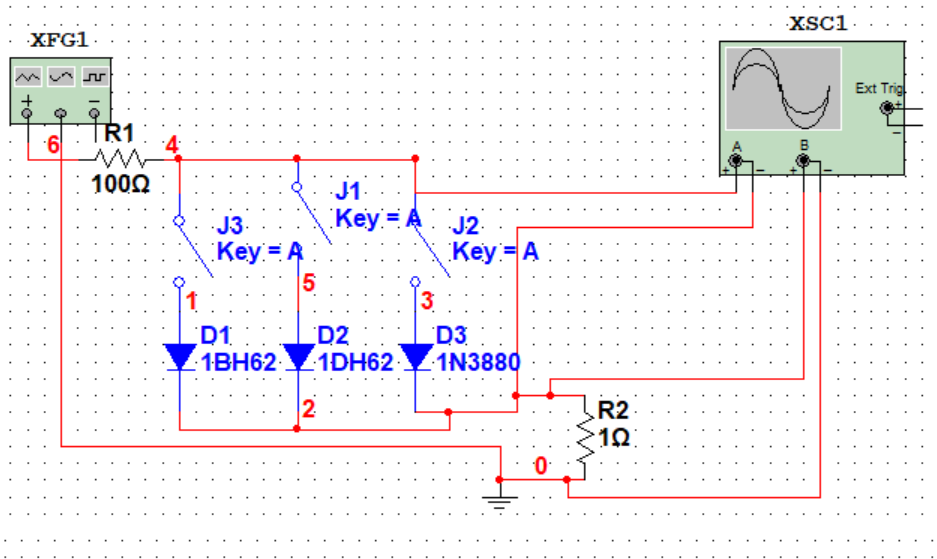
\includegraphics[width=0.8\linewidth]{Схема.png}

\caption{CСхема, що використовувалась у роботі}

\label{fig:mpr}

\end{figure}

\newpage
\subsection{Діод 1}
\begin{figure}[ht]

\centering

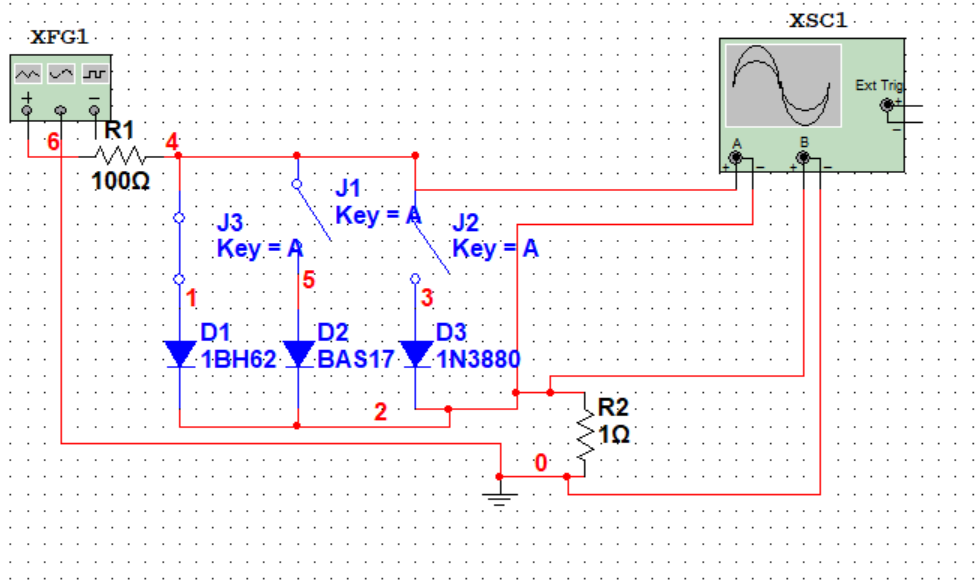
\includegraphics[width=0.6\linewidth]{Діод1Схема.png}

\caption{Схема}

\label{Diod1Shema}

\end{figure}

\begin{figure}[ht]

\centering

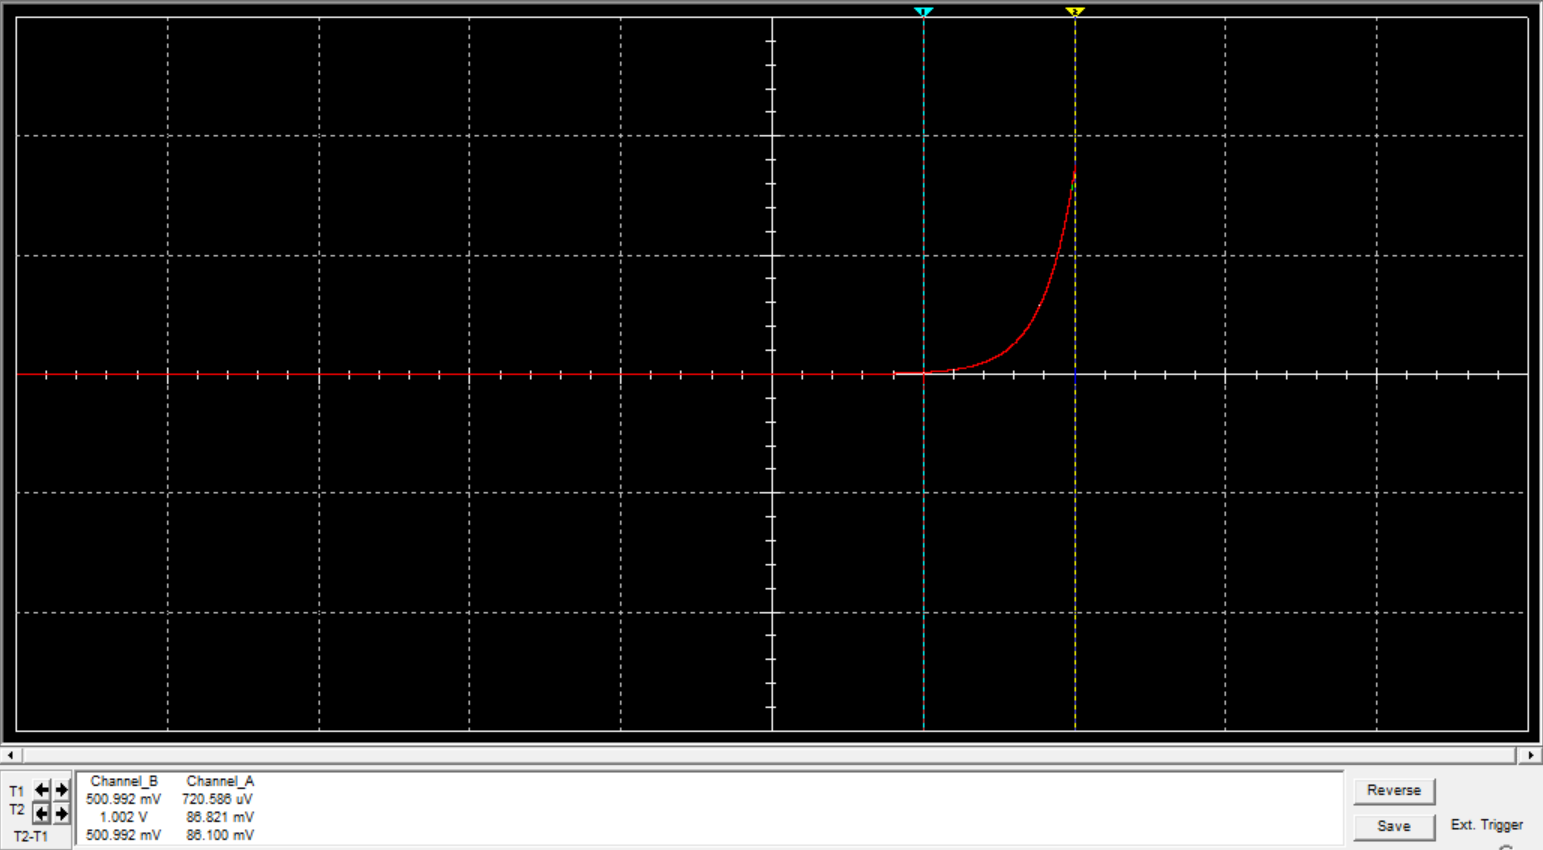
\includegraphics[width=0.75\linewidth]{Діод1Осцилограф.png}

\caption{Результати вимірів}

\label{Diod1Osc}

\end{figure}

\begin{figure}[ht]

\centering

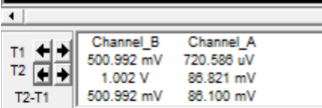
\includegraphics[width=0.3\linewidth]{Діод1Рез.png}

\caption{Результати вимірів}

\label{Diod1Rez}

\end{figure}

Оскільки канал А виводить напругу на резисторі опором $1  \Omega $, можемо вважати, що отримані значення - сила струму у колі.

\newpage
\subsection{Діод 2}
\begin{figure}[ht]

\centering

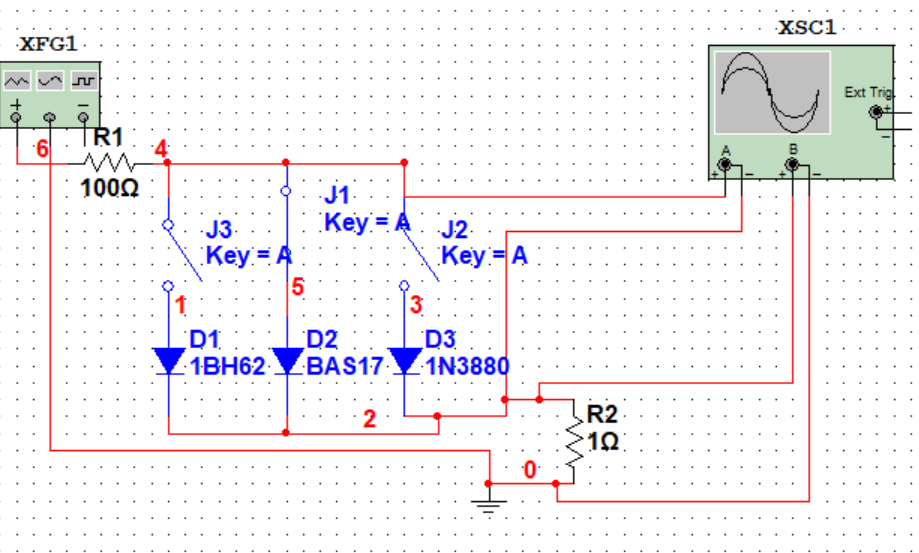
\includegraphics[width=0.6\linewidth]{Діод2Схема.png}

\caption{Схема}

\label{Diod2Shema}

\end{figure}

\begin{figure}[ht]

\centering

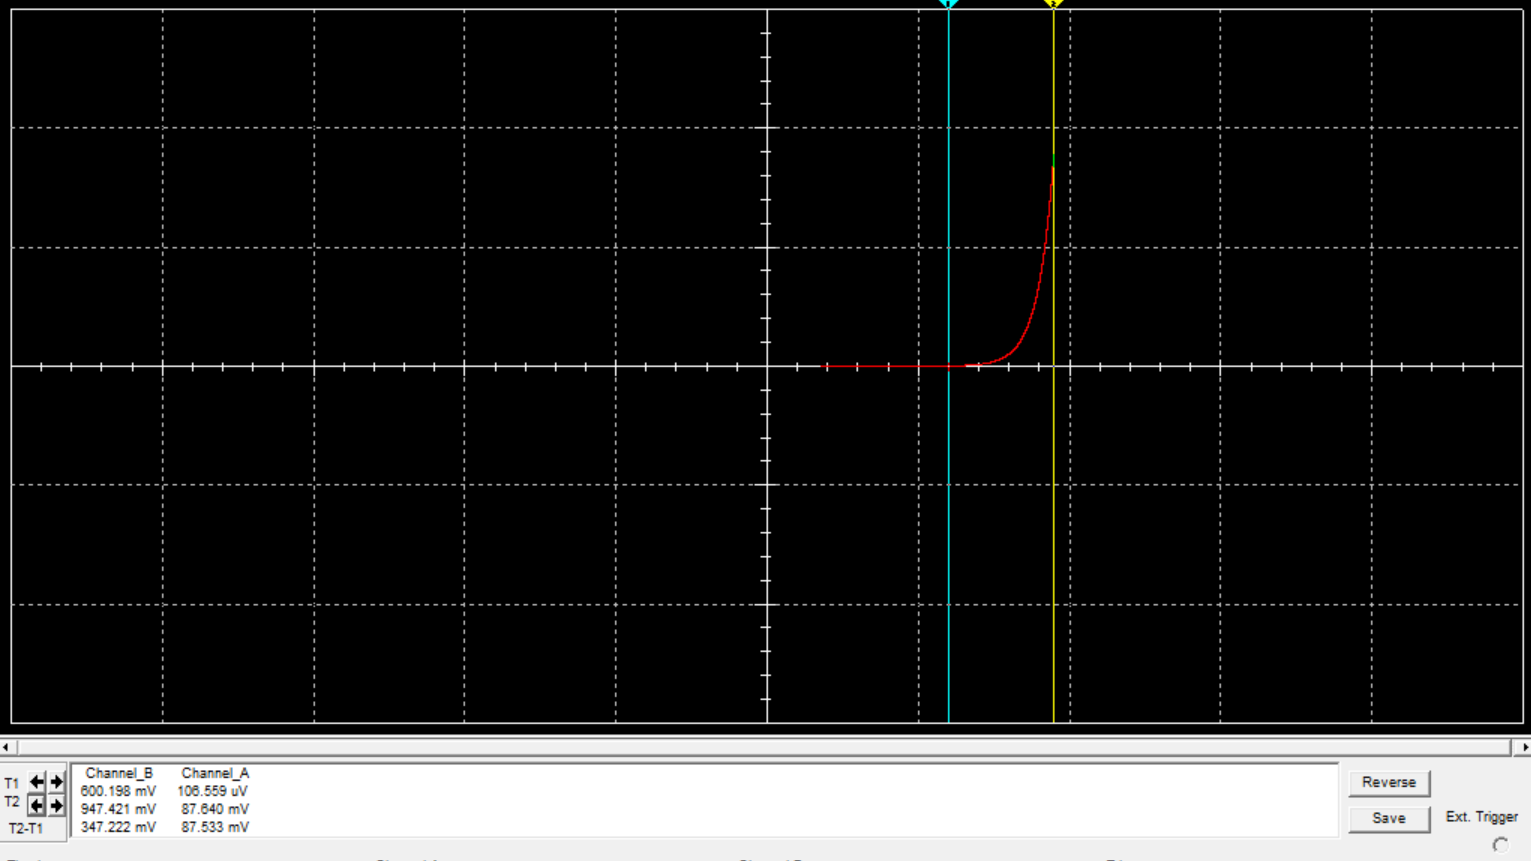
\includegraphics[width=0.75\linewidth]{Діод2Осцилограф.png}

\caption{Результати вимірів}

\label{Diod2Osc}

\end{figure}

\begin{figure}[ht]

\centering

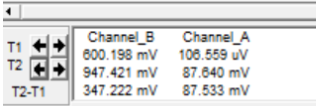
\includegraphics[width=0.3\linewidth]{Діод2Рез.png}

\caption{Результати вимірів}

\label{Diod2Rez}

\end{figure}

\newpage
\subsection{Діод 3}
\begin{figure}[ht]

\centering

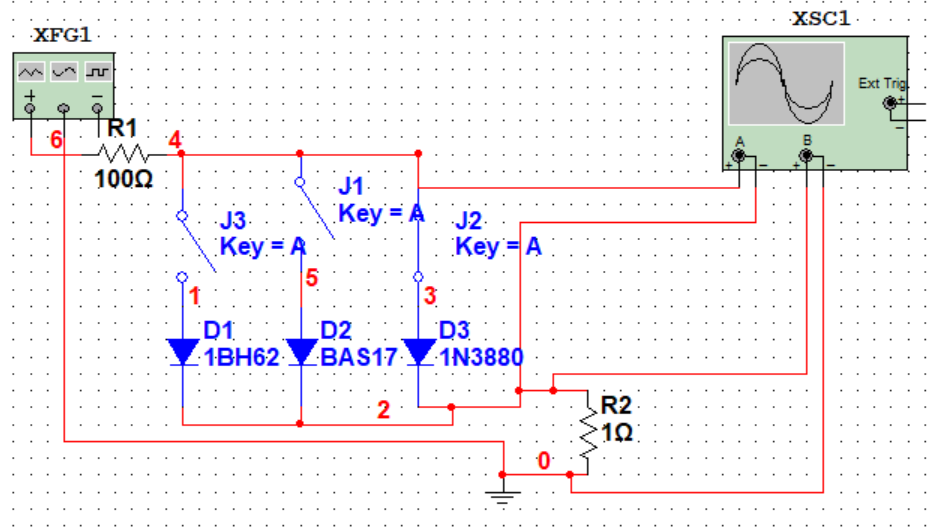
\includegraphics[width=0.6\linewidth]{Діод3Схема.png}

\caption{Схема}

\label{Diod3Shema}

\end{figure}

\begin{figure}[ht]

\centering

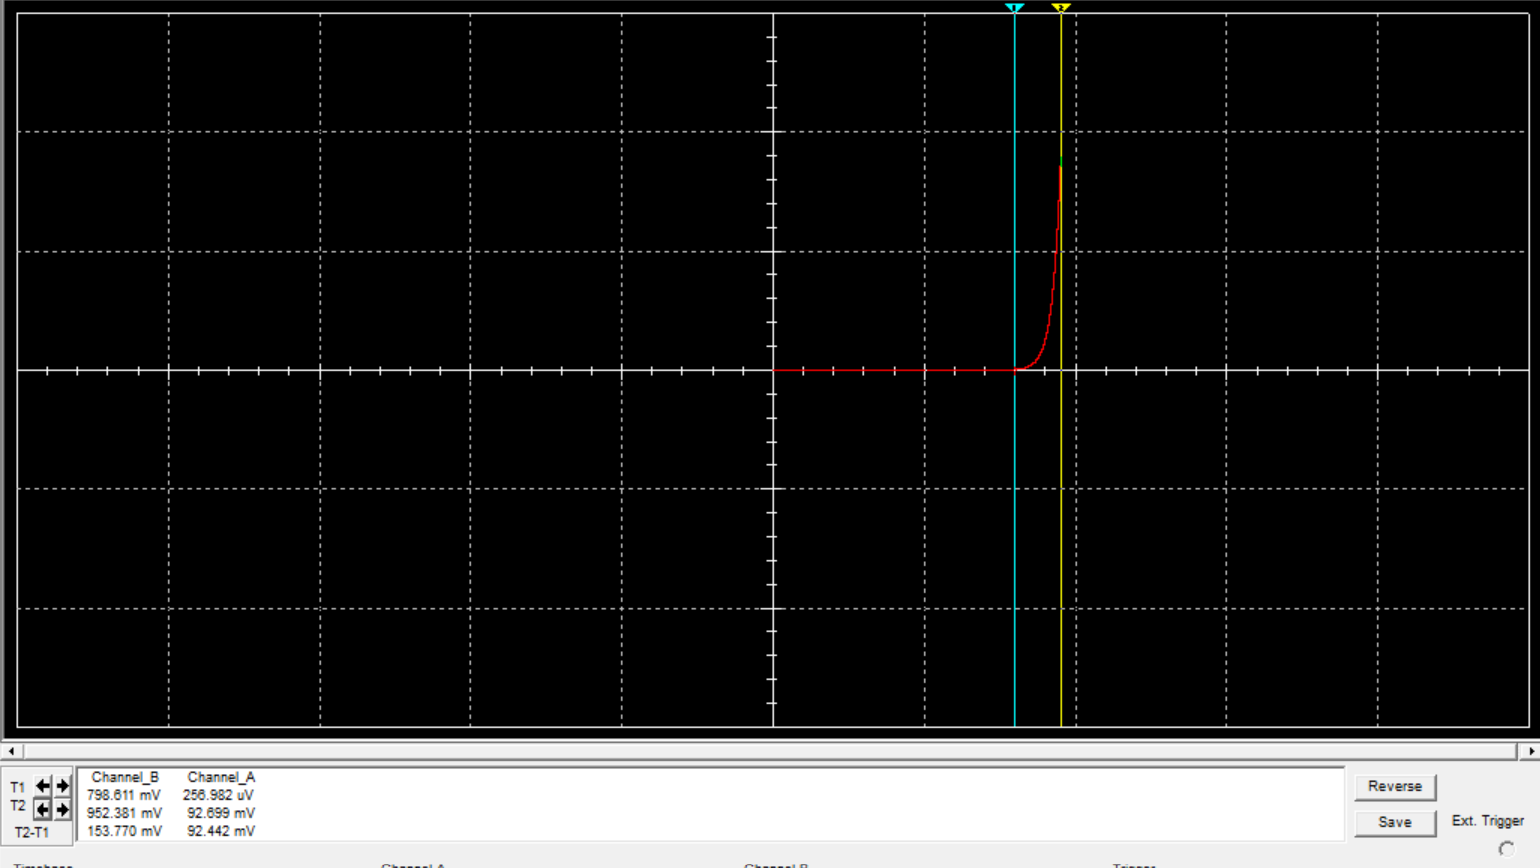
\includegraphics[width=0.75\linewidth]{Діод3Осцилограф.png}

\caption{Результати вимірів}

\label{Diod3Osc}

\end{figure}

\begin{figure}[ht]

\centering

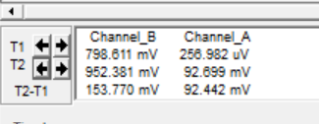
\includegraphics[width=0.3\linewidth]{Діод3Рез.png}

\caption{Результати вимірів}

\label{Diod3Rez}

\end{figure}

\newpage
\subsection{Робота з Arduino}
\input{Ардуино}
\newpage






\section{Відповіді на контрольні запитання}
\subsection{Напівпровідники $n$– та $p$–типу. Основні та неосновні носії заряду в таких напівпровідниках.}
\qquad   електрони в матеріалі $n$-типу називають \emph{основними носіями} заряду, а дірки – \emph{неосновними носіями заряду}. В матеріалі $p$-типу – навпаки: дірки є \emph{основними носіями} заряду, а електрони – \emph{неосновними}.\\
Для того, щоб отримати напівпровідник n-типу, власний напівпровідник легують донорами. Здебільшого це атоми, які мають на валентній оболонці на один електрон більше, ніж атоми напівпровідника, який легується.\\
Напівпровідники p-типу отримують методом легування власних напівпровідників акцепторами. Тобто атомами, що мають на один електрон менше, ніж атоми напівпровідника.
\subsection{$p$–$n$-перехід. Власне електричне поле переходу. Контактна різниця
потенціалів. Дифузійний та дрейфовий струми..}
\qquad
При встановленні контакту між двома напівпровідниковими матеріалами, матеріал n-типу буде втрачати негативний заряд і набувати позитивного заряду, а матеріал p-типу, навпаки, буде втрачати позитивний заряд і набувати негативного заряду. В результаті в області контакту буде виникати електричне поле, яке буде протидіяти подальшому переходу
електронів в p-область та дірок в n-область, і між матеріалом n-типу і матеріалом p-типу виникатиме різниця потенціалів. Ця різниця потенціалів називається контактною різницею потенціалів $\phi_k$, а вищезгадане електричне поле – полем p–n-переходу $E_{n-p}$. \\В основі дифузійного струму лежить хаотичний рух носіїв заряду, при якому вони переходять із області, де їх більше у область, де їх менше. Дрейфовий струм — електричний струм, зумовлений рухом носіїв електричного заряду під дією електричного поля.
\subsection{Пряме та зворотне включення $p$–$n$-переходу. Рух основних та неосновних
носіїв через $p$–$n$-перехід під дією прямої та зворотної напруги}
\qquad
Якщо до p–n-переходу прикласти зовнішню напругу у зворотному
напрямку ($U$ < 0) і збільшувати її, то струм основних носіїв прямуватиме
до нуля і при достатньо великих значеннях зворотної напруги повний
струм І (його ще називають зворотним струмом) буде повністю
визначатися струмом неосновних носіїв і перестане залежати від $U$.
\subsection{Вольт-амперна характеристика (ВАХ) випрямлювального діода, її залежність від температури. Застосування випрямлювальних діодів в техніці.}
\qquad
Струм $I$ залежить від температури та ширини забороненої зони
напівпровідника:$I = I_0 e^{\frac{E_g}{kT}} $ , де $I_0$ — множник, що слабко залежить від
температури. Діоди, що мають таку ВАХ, називають випрямлювальними
(англ. rectifier diode) і використовують у пристроях випрямлення,
обмеження, детектування. Найпотужніші з них здатні працювати при
значеннях прямого струму до кількох тисяч ампер і витримувати без
пробою зворотні напруги в десятки кіловольт.
\subsection{Оборотний та необоротний електричний пробій $p$–$n$-переходу. ВАХ
стабілітрона. Застосування стабілітронів. }
При великих зворотних напругах $p$–$n$-перехід "пробивається" і через
нього протікає дуже великий струм. Пробій є відновлюваним, доки
теплова потужність, розсіювана на $p$–$n$-переході, не перевищує
припустимої, при якій відбувається його руйнування. Ця ділянка ВАХ, що
відповідає зворотній напрузі, використовується на практиці в пристроях
стабілізації напруги, а діоди, що мають таку ділянку, називають
стабілітронами. Напругу пробою можна регулювати
технологічно (як правило, варіюванням концентрації домішок в $p$- і nобластях) в широких межах – від одиниць до сотень вольт. Для
стабілізації напруги використовується і вертикальна ділянка ВАХ в
прямому напрямку.
\subsection{Тунельний ефект. Енергетична діаграма та ВАХ тунельного діода.
Застосування тунельних діодів}
Якщо виготовити $p$–$n$-перехід з сильнолегованого напівпровідника (з
великою концентрацією домішок), то перехід стане тонким і носії заряду
зможуть "просочуватися" (тунелювати) через область $p$–$n$-переходу при
прикладанні невеликої як зворотної, так і прямої напруги. Діоди з таким
$p$–$n$- переходом називаються тунельними. ВАХ таких
діодів поблизу початку координат ($U$ = 0) являє собою відрізок прямої,
тобто подібна до ВАХ звичайного резистора. Важливою особливістю
ВАХ тунельних діодів є наявність на її прямій гілці ділянки з від’ємним
диференціальним опором: $R_dif$ = $\frac{\delta U}{\delta I}$ < 0 (пунктирна лінія на Рис. 9), що
дозволяє використовувати їх як підсилювачі та генератори електричних
коливань надвисокочастотного діапазону (до десятків гігагерц). Такі діоди
використовуються також як швидкодійні перемикачі, а також як елементи
пам’яті в запам’ятовувальних пристроях з двійковим кодом.
\subsection{Випромінювальна рекомбінація носіїв заряду в напівпровідниках.
Принцип роботи і застосування світлодіодів.}
У будь-якому прямозміщеному (включеному в прямому напрямку) p–nпереході при протіканні струму має місце рекомбінація носіїв заряду, в
тому числі й випромінювальна, тобто з народженям фотонів.
Випромінювально рекомбінує лише частина носіїв. І лише частина
фотонів, уникнувши поглинання в самому діоді, може вийти назовні. Для
створення практично придатного світловипромінювального діода
(світлодіода) необхідні матеріали з
високою імовірністю випромінювальної рекомбінації. Якщо для випрямлювальних діодів використовуються переважно германій $Ge$ і
кремній $Si$, то матеріалом для cвітлодіодів є арсенід галію $GaAs$, фосфід
галію $GaP$ і потрійні напівпровідникові сполуки на їх основі, а також
карбід кремнію $SiC$. Сьогодні більш ефективними є світлодіоди, у яких
використовуються не $p$–$n$-переходи, а так звані гетеропереходи – переходи
між двома напівпровідниковими матеріалами з різною шириною
забороненої зони. Оскільки енергія фотонів випромінювання (колір
свічення) близька до ширини забороненої зони напівпровідника, то на
основі перелічених напівпровідникових матеріалів були створені
світлодіоди, що випромінюють у всій видимій, інфрачервоній та ближній
ультрафіолетовій областях спектра.
\subsection{Внутрішній фотоефект у напівпровідниках. Принцип роботи і
застосування фотодіодів. Сонячні батареї}
Внутрішній фотоефект -
перерозподіл електронів по енергетичних рівнях у діелектриках я
напівпровідниках (але не в металах) під дією світла. Якщо енергія кванта
hv падаючого світла перевищує ширину забороненої зони в діелектрику
або напівпровіднику, то електрон, що поглинув квант, переходить із
валентної зони в зону провідності. У результаті цього переходу
утворюється пара носіїв: у зоні провідності електрон, а у валентній зоні -
дірка. Таким чином, у зоні провідності з'являються носії заряду, і при
включенні напівпровідника в ланцюг по ній буде протікати струм або при
додатку зовнішнього електричного поля буде протікати струм, що
змінюється залежно від освітленості. Фотовольтаїчний модуль – це
спеціальна конструкція, яка складається з набору взаємозв’язаних
фотоелектричних комірок. Кожна з цих комірок, або селів (cell – анг.
комірка), виготовлена з певного напівпровідника, наприклад кремнію,
який в переважній більшості застосовується для створення сонячних
панелей, оскільки демонструє наразі найвищі показники продуктивності.
Коли сонячні промені потрапляють на цей напівпровідник, то він починає
нагріватися, частково поглинаючи виділену від променів енергію. Фотони
світла «вибивають» електрони з загальної атомної структури напівпровідника, і вільні електрони формують заряд.

\section{Список використаної літератури}
\begin{enumerate}
  \item Методичні вказівки до практикуму «Основи радіоелектроніки» для студентів фізичного факультету / Упоряд. О.В.Слободянюк
  \item Ю.О.Мягченко, В.М.Кравченко.- К.: Поліграфічний центр «Принтлайн», 2007.- 120 с.
  \item Ю.О. Мягченко, Ю.М. Дулич, А.В.Хачатрян “Вивчення
радіоелектронних схем методом комп’ютерного моделювання” :
Методичне видання. – К.: 2006.- с
\end{enumerate}












\end{document} % Конец текста.
